\documentclass[sigconf]{acmart}

\usepackage{booktabs} % For formal tables

\usepackage{graphicx}
\usepackage{here} % [H]とするとその場所に配置されるらしい

% Copyright
%\setcopyright{none}
%\setcopyright{acmcopyright}
%\setcopyright{acmlicensed}
\setcopyright{rightsretained}
%\setcopyright{usgov}
%\setcopyright{usgovmixed}
%\setcopyright{cagov}
%\setcopyright{cagovmixed}


% % DOI
% \acmDOI{10.475/123_4}
% 
% % ISBN
% \acmISBN{123-4567-24-567/08/06}
% 
% %Conference
% \acmConference[AVI2018]{ACM Woodstock conference}{July 2018}
%               {Rome, Italy}
% \acmYear{2018}
% \copyrightyear{2018}
% 
% 
% \acmArticle{4}
% \acmPrice{15.00}

% These commands are optional
%\acmBooktitle{Transactions of the ACM Woodstock conference}
% \editor{Jennifer B. Sartor}
% \editor{Theo D'Hondt}
% \editor{Wolfgang De Meuter}


\begin{document}
\title{EpisoDAS - DAS-based password generation \\
using episodic memories}
% \titlenote{Produces the permission block, and copyright information}

\author{Toshiyuki Masui}
% \authornote{Is this necessary?.}
\orcid{1234-5678-9012}
\affiliation{%
  \institution{Keio University}
  \streetaddress{Endo}
  \city{Fujisawa}
  \state{Kanagawa}
  \postcode{43017-6221}
}
\email{masui@masui.org}

\renewcommand{\shortauthors}{T. Masui}

\begin{abstract}

We introduce a simple and powerful visual interaction technique for
managing strong passwords.
%
Passwords have been used for qauthentication for decades, but
appropriate handling of passwords is difficult because people can
easily forget passwords and they can be easily cracked.
%
To make the authentication process easier, various visual interaction
methods have been proposed, including the DAS (draw-a-secret)
method. Using DAS, users can log into various services just by drawing
a secret pattern on the screen.
%
Using a DAS-based authentication method, users can quickly log into a
service without typing a password. However, remembering complex secret
patterns can be as difficult as remembering passwords. We developed
EpisoDAS, with which users can generate strong passwords based on
their secret episodic memories with a simple DAS interface.
%
users can use secret patterns for authentication, based on their
secret episodic memories which they cannot easily forget.

\end{abstract}

\maketitle

\section{Introduction}

Passwords have been used as a means of authenticating to Web services
and applications for a long time, and remain the most popular
authentication method on the Internet.
Since short passwords are easily guessable by attackers and using the
same password for multiple services is unsafe, a different long
password should be used for each service a person uses.
However, remembering numerous long passwords is almost impossible for
ordinary humans.

However, password-based authentication is still the most convenient
and widely deployed method \cite{Bonneau:ReplacePasswords}, and is not
expected to disappear any time soon \cite{Herley:2009:PSS:1601990.1602010}.
%
To tackle this problem,
we have been proposing the \textit{EpisoPass} password generator with which 
users can generate strong passwords easily
based only on a user's secret and unforgettable episodic memories.

% For this reason, we believe that it is far better to ``generate''
% something for the authentication, based on a user's episodic
% memories. This has the benefit that unlike a password, a person is
% highly unlikely to forget such episodic memories.

\begin{figure}[H]
  \centerline{\includegraphics[width=12cm,bb=-300 -100 1222 1014]{figures/episopass.png}}
  \caption{EpisoPass}
  \label{EpisoPass}
\end{figure}

Password generation on EpisoPass is performed through the following steps:

\begin{enumerate}
\item A user registers multiple question texts related to their own personal
secret unforgettable episodic memories. For each question they must provides
a single correct answer and multiple additional incorrect answers.

\item The user provides a long ``seed string'' for each service that requires
a password.

\item EpisoPass shows the questions and answers to the user allowing
them to select the correct answer for each question.
Based on the user's selections,
EpisoPass substitutes characters in the seed string and generates a
strong password candidate string.
After selecting all of the correct answers,
the user copies the calculated string
and registers it as the password for the service.
\end{enumerate}

The biggest advantage of using EpisoPass is that
users don't have to remember strong password strings.
%
Users of EpisoPass can save the questions and answers
wherever is convenient. They can
then easily generate passwords by running
EpisoPass and answering the questions.
%
If a question is based on old unforgettable episodic memory,
there is little chance of losing the password for a service
as long as the seed string and questions are available.
%
Answering to many questions takes much longer time than typing a
remembered password, so people may prefer typing password
rather than using EpisoPass if they have to log in to a service frequently.


For the people who don't like to use passwords for authentication,
various types of authentication methods have been proposed.
Especially, visual authentication methods
like graphical passwords\cite{Biddle:2012:GPL:2333112.2333114,GraphicalPasswords}
and Draw-a-Secret (DAS) \cite{DAS} are promising approaches, because
people can remember visual patterns easier than passwords.

% \begin{figure}[H]
%   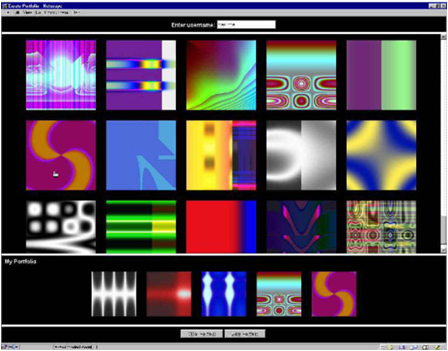
\includegraphics[width=8cm,bb=0 0 448 351]{figures/Dejavu.png}
%   \caption{D\'{e}j\`{a} Vu}
%   \label{fig:sample}
% \end{figure}

\begin{figure}
  % 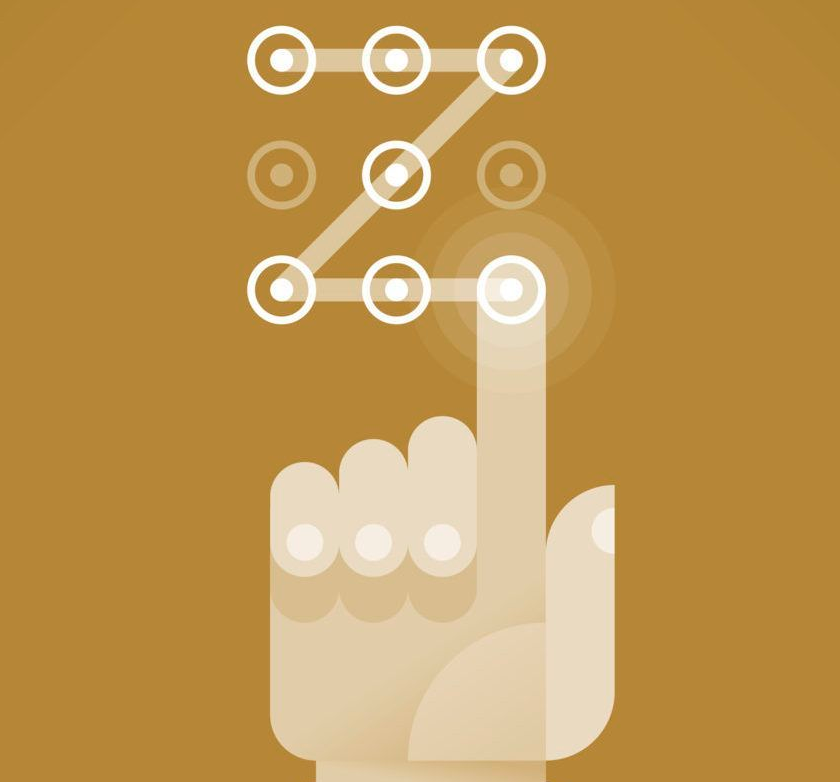
\includegraphics[width=8cm,bb=0 0 840 792]{figures/DAS.png}
  % 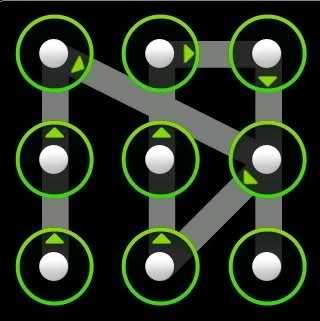
\includegraphics[width=8cm,bb=0 0 320 321]{figures/DASexample.jpg}
  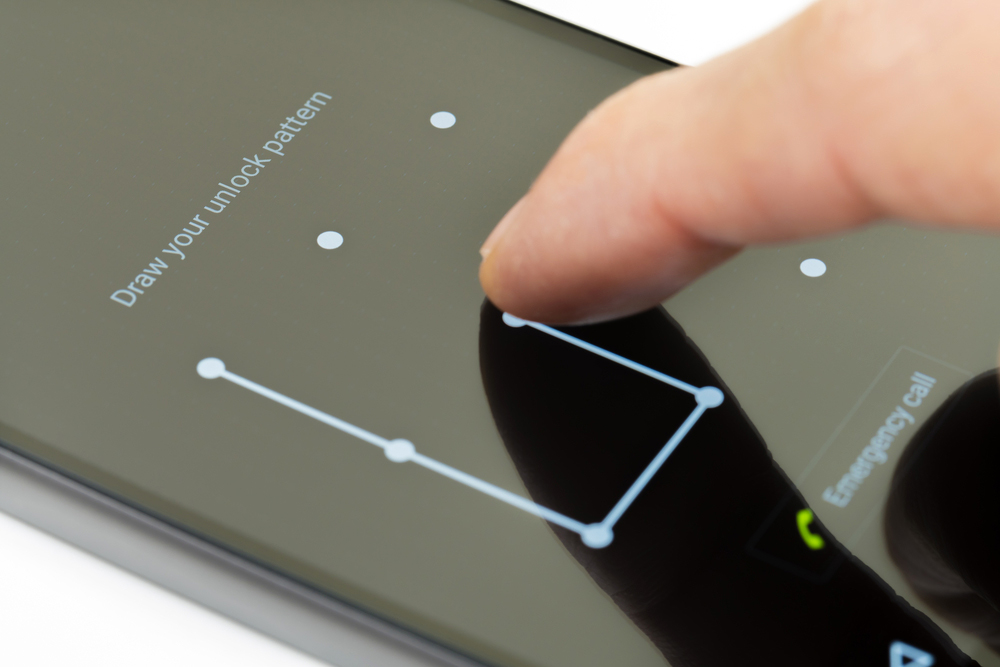
\includegraphics[width=12cm,bb=0 0 1000 667]{figures/AndroidLock.jpg}
  \caption{An example DAS pattern for Android.}
  \label{AndroidLock}
\end{figure}

Visual authentication methods have better characteristics than
password-based authentication, but
they are either more fragile to attacks
or remembering is difficult.

We propose a new visual password generation system \textit{EpisoDAS},
which have the advantages of both EpisoPass and DAS-based methods.

\section{EpisoDAS}

EpisoDAS is a visual authentication interface
based on the user's episodic memories.
Like EpisoPass,
EpisoDAS displays a list of questions to the user and
ask the user to choose the most appropriate answers.
EpisoDAS then generates a password string based on the user's selections.
%
% with which users can generate strong password based on their
% memory of visual patterns and episodic memories.
% Users can either select answers based on the user's secret episodic memories or
% draw a secret pattern represented by the pattern of selected answers.
% 
% Thus, users can recognize EpisoDas as a DAS system or
% use it as an implementation of EpisoPass.
%
The candidate answers are shown to the user as a grid of buttons,
and the user can select the most appropriate answer
by clicking one of the buttons in the grid.

If the series of correct answers form a special pattern
that the user can remember,
the user can select the series of correct answers quickly
just like using other DAS systems.

% http://episopass.com/Amazon_john@example.com/Amazon123456
% http://episopass.com/Amazon_john@example.com.html

\begin{figure}[H]
  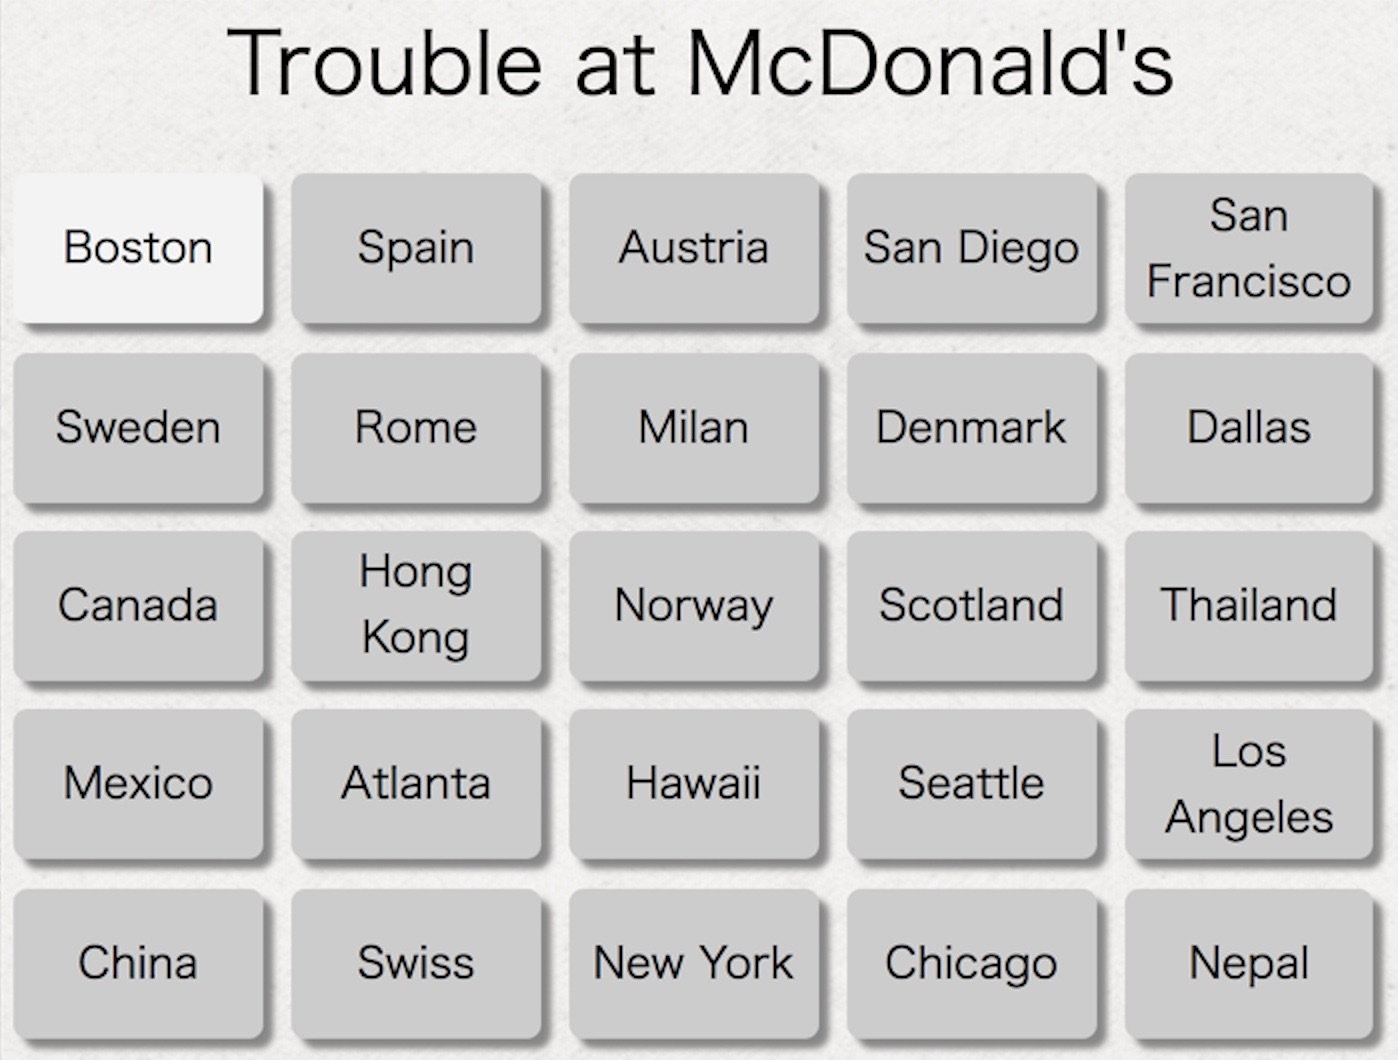
\includegraphics[width=12cm,bb=0 0 1398 1060]{figures/EpisoDAS1.jpg}
  \caption{First question}
  \label{EpisoDAS1}
\end{figure}

Figure \ref{EpisoDAS1} shows
the initial screen of an EpisoDAS session.
% how a user can generate a password from his episodic memories.
%
If the user remembers that he had trouble at a MacDonald's in Boston in the past,
he would click ``Boston'', and the next question (Figure \ref{EpisoDAS2}) is displayed.
The contents and the order of the questions
do not depend on the user's actions, and
the user cannot tell whether he has selected a right answer.

\begin{figure}[H]
  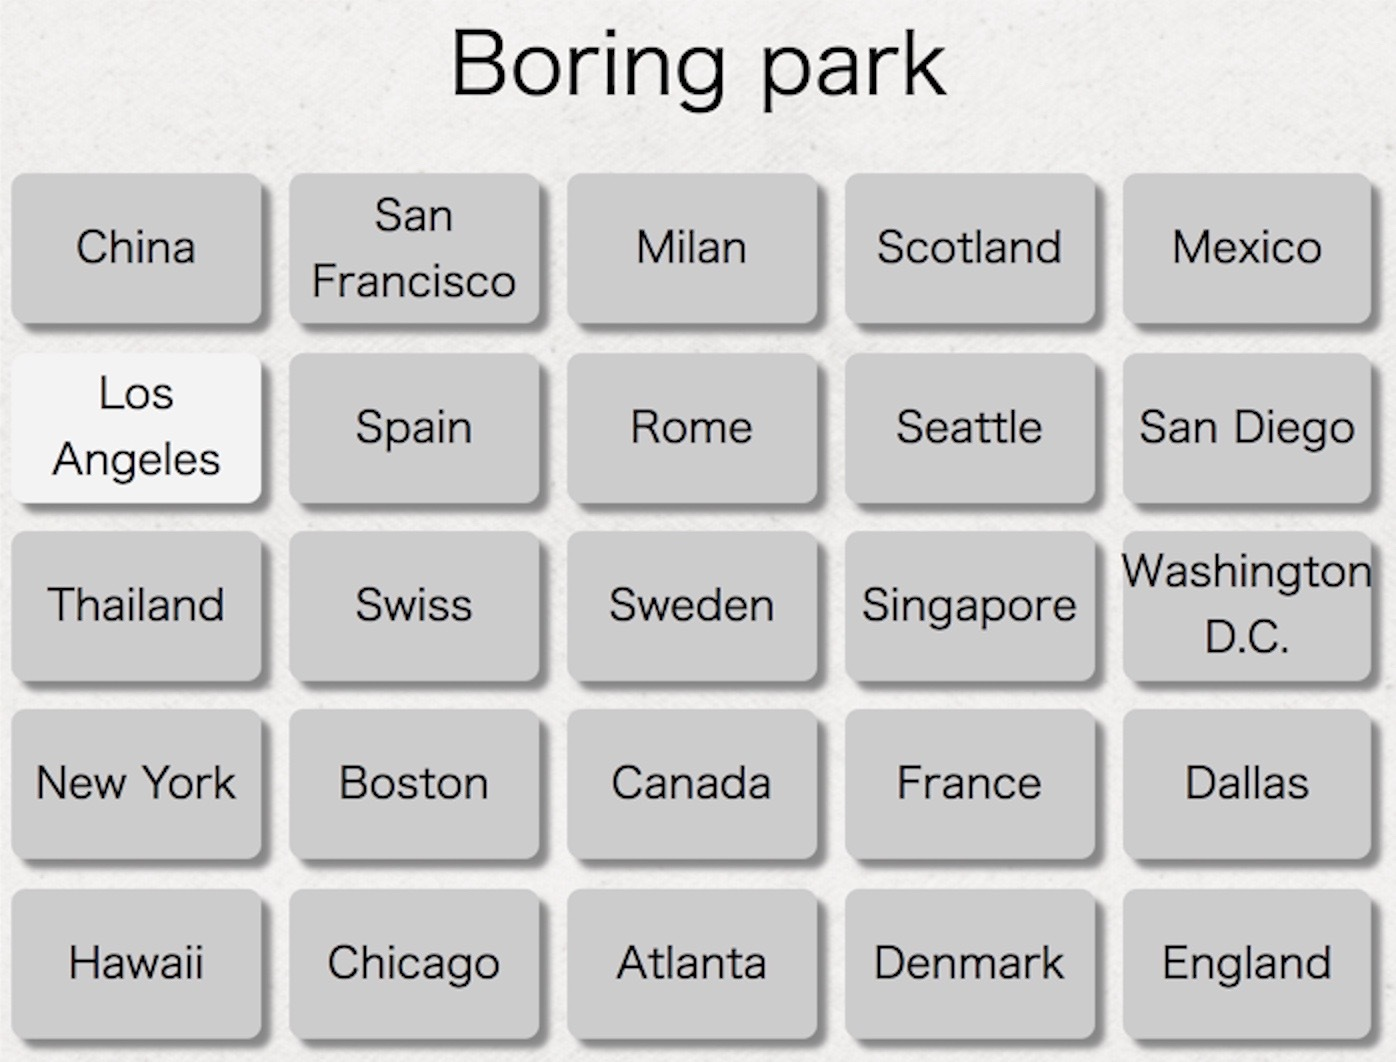
\includegraphics[width=12cm,bb=0 0 1396 1062]{figures/EpisoDAS2.jpg}
  \caption{Second question}
  \label{EpisoDAS2}
\end{figure}

If he remembers that he had a bad time at Los Angeles
after reading the question in Figure \ref{EpisoDAS2},
he would click ``Los Angeles'' and proceed to the third question.
%
After repeating the slection process ten times,
the user can get his password
calculated from his selections. (Figure \ref{Result})

\begin{figure}[H]
  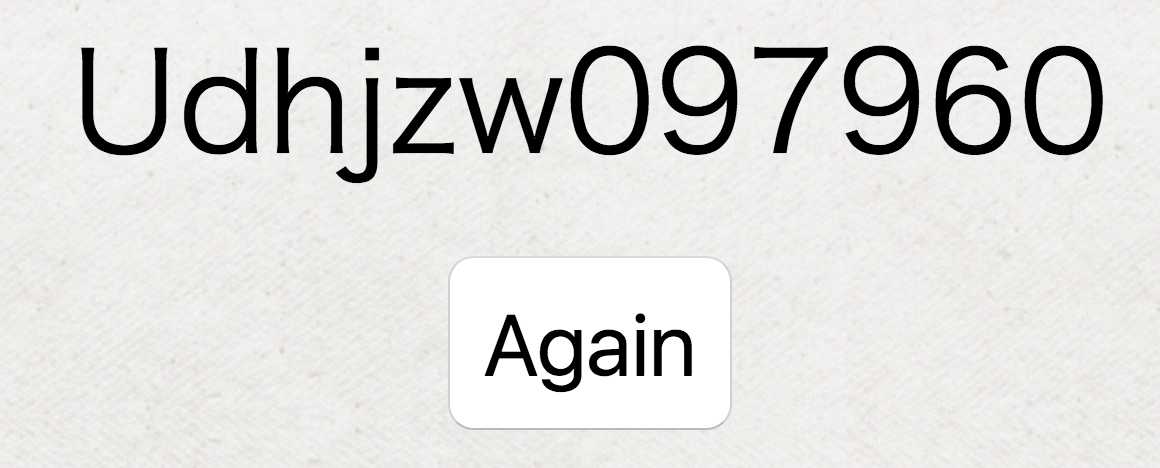
\includegraphics[width=12cm,bb=0 0 1160 468]{figures/result.png}
  \caption{Generated password}
  \label{result}
\end{figure}

If the series of right-answer buttons form a special DAS pattern,
% If the series of buttons are aligned next to each others,
the user can drag the pointing device like
Figure \ref{draw} and quickly get the generated
password without clicking buttons.
%
The candidate answers change according to the drag or click of the
pointing device, and the user can mix the dragging and clicking actions
at any point.

\begin{figure}[H]
  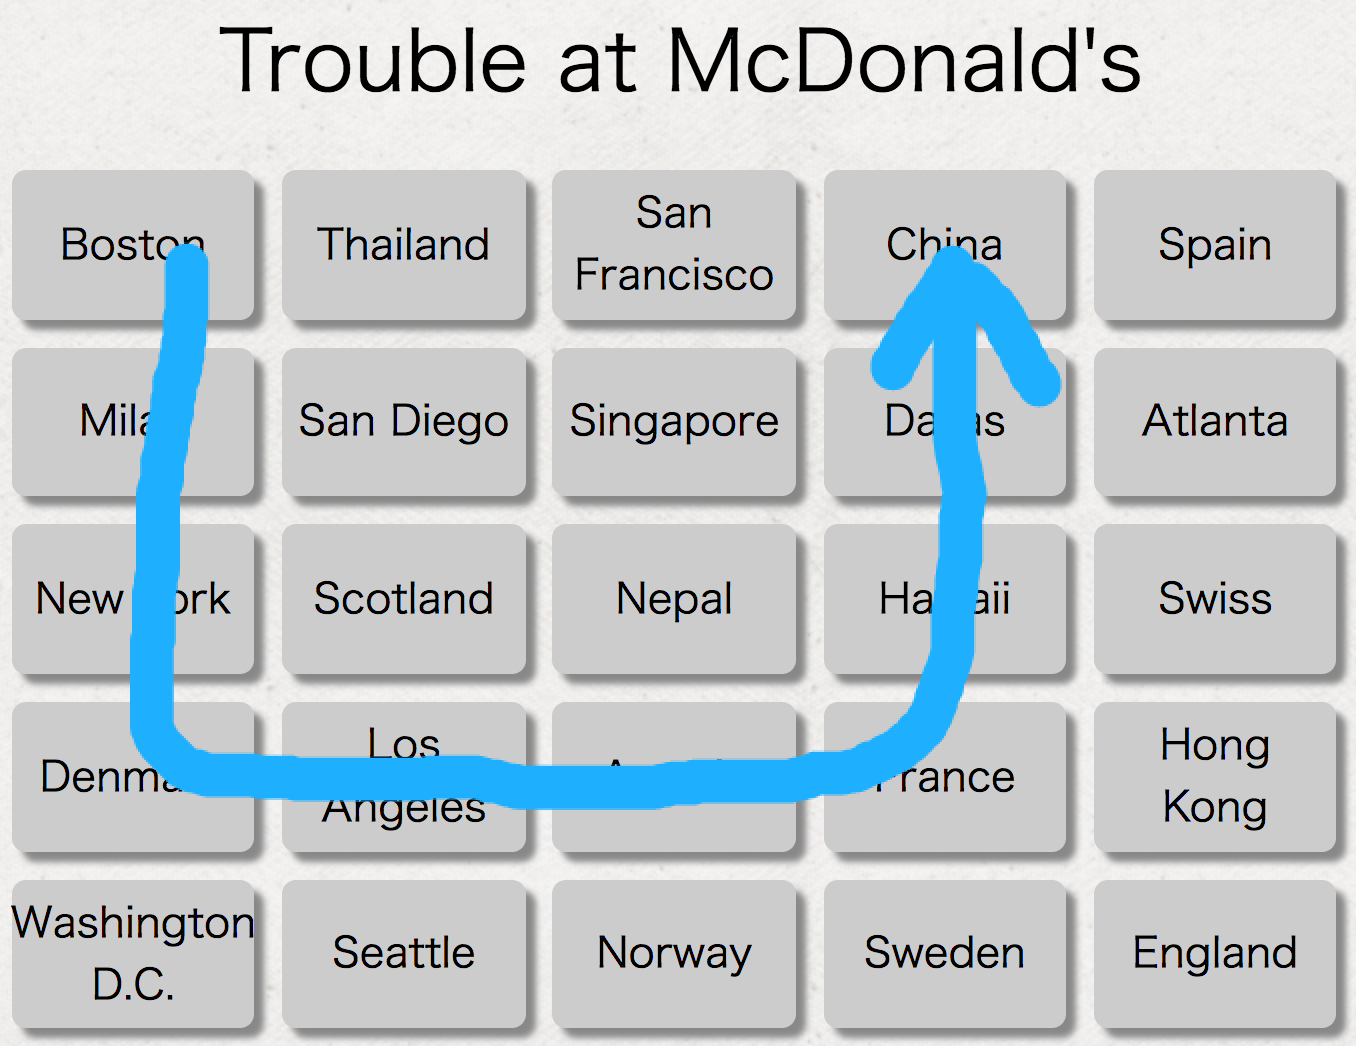
\includegraphics[width=12cm,bb=0 0 1130 1236]{figures/draw.png}
  \caption{Drawing a secret pattern}
  \label{draw}
\end{figure}

The drawing action by the user is close to the actions
used on conventional DAS systems.
Users can quickly generate his password for authentication
just by
drawing a pattern on the EpisoDAS screen.

EpisoDAS can be used for generating passwords for any kind of systems and
services, but it is most useful when used on a login window.
Figure \ref{Amazon} shows how a user can use EpisoDAS when
he wants to log in to Amazon.com.
If the EpisoDAS extension is installed on the browser,
an EpisoDAS window appears when the user enters his
email address and clicks the password field at Amazon.com.
After selecting answers, a password is generated and pasted
into the password field, making the user to log in without typing a password.

% Figure \ref{Amazon} shows how a user can use EpisoDAS on a login page,
% using a browser extension software.
% The extension shows a EpisoDAS window when a user tries to log into
% an Web service, and after the user selects the right answers,
% a password is generated from the input and pasted in to the
% password text box.

\begin{figure}[H]
  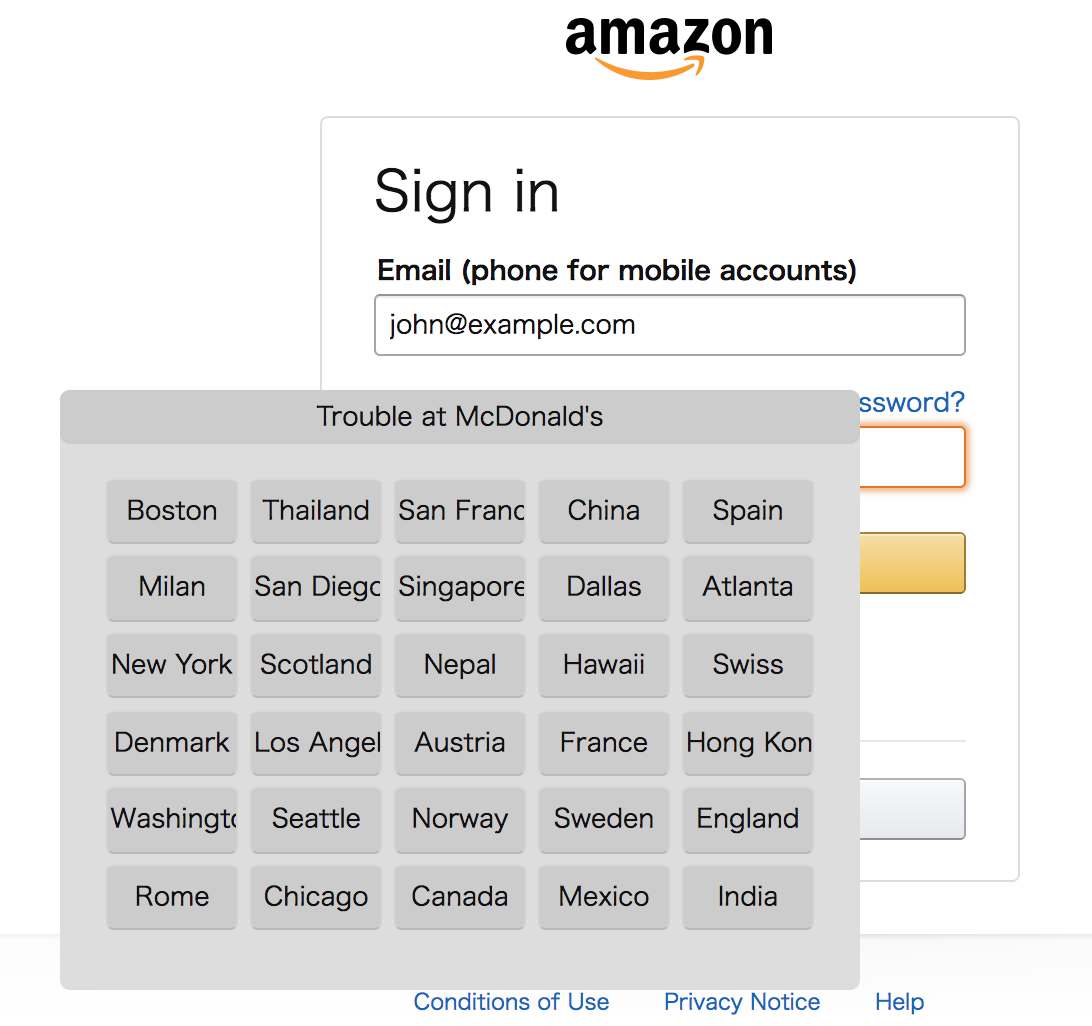
\includegraphics[width=12cm,bb=0 0 1092 1026]{figures/Amazon.png}
  \caption{Login to Amazon.com}
  \label{Amazon}
\end{figure}

The data used in the above example is retrieved from the EpisoDAS database
on the Web, using the name of the service (e.g. \texttt{Amazon})
and the user id (e.g. \texttt{joe@example.com}).

\section{Registration}

\subsection{Registering a DAS pattern}

EpisoDAS is the predecessor of the EpisoPass system,
and questions and answers should be registered on the EpisoPass system.
After registering questions and answer candidates,
a user can register a DAS pattern so that
answer candidates are easily selected on EpisoDAS.

\begin{figure}[H]
  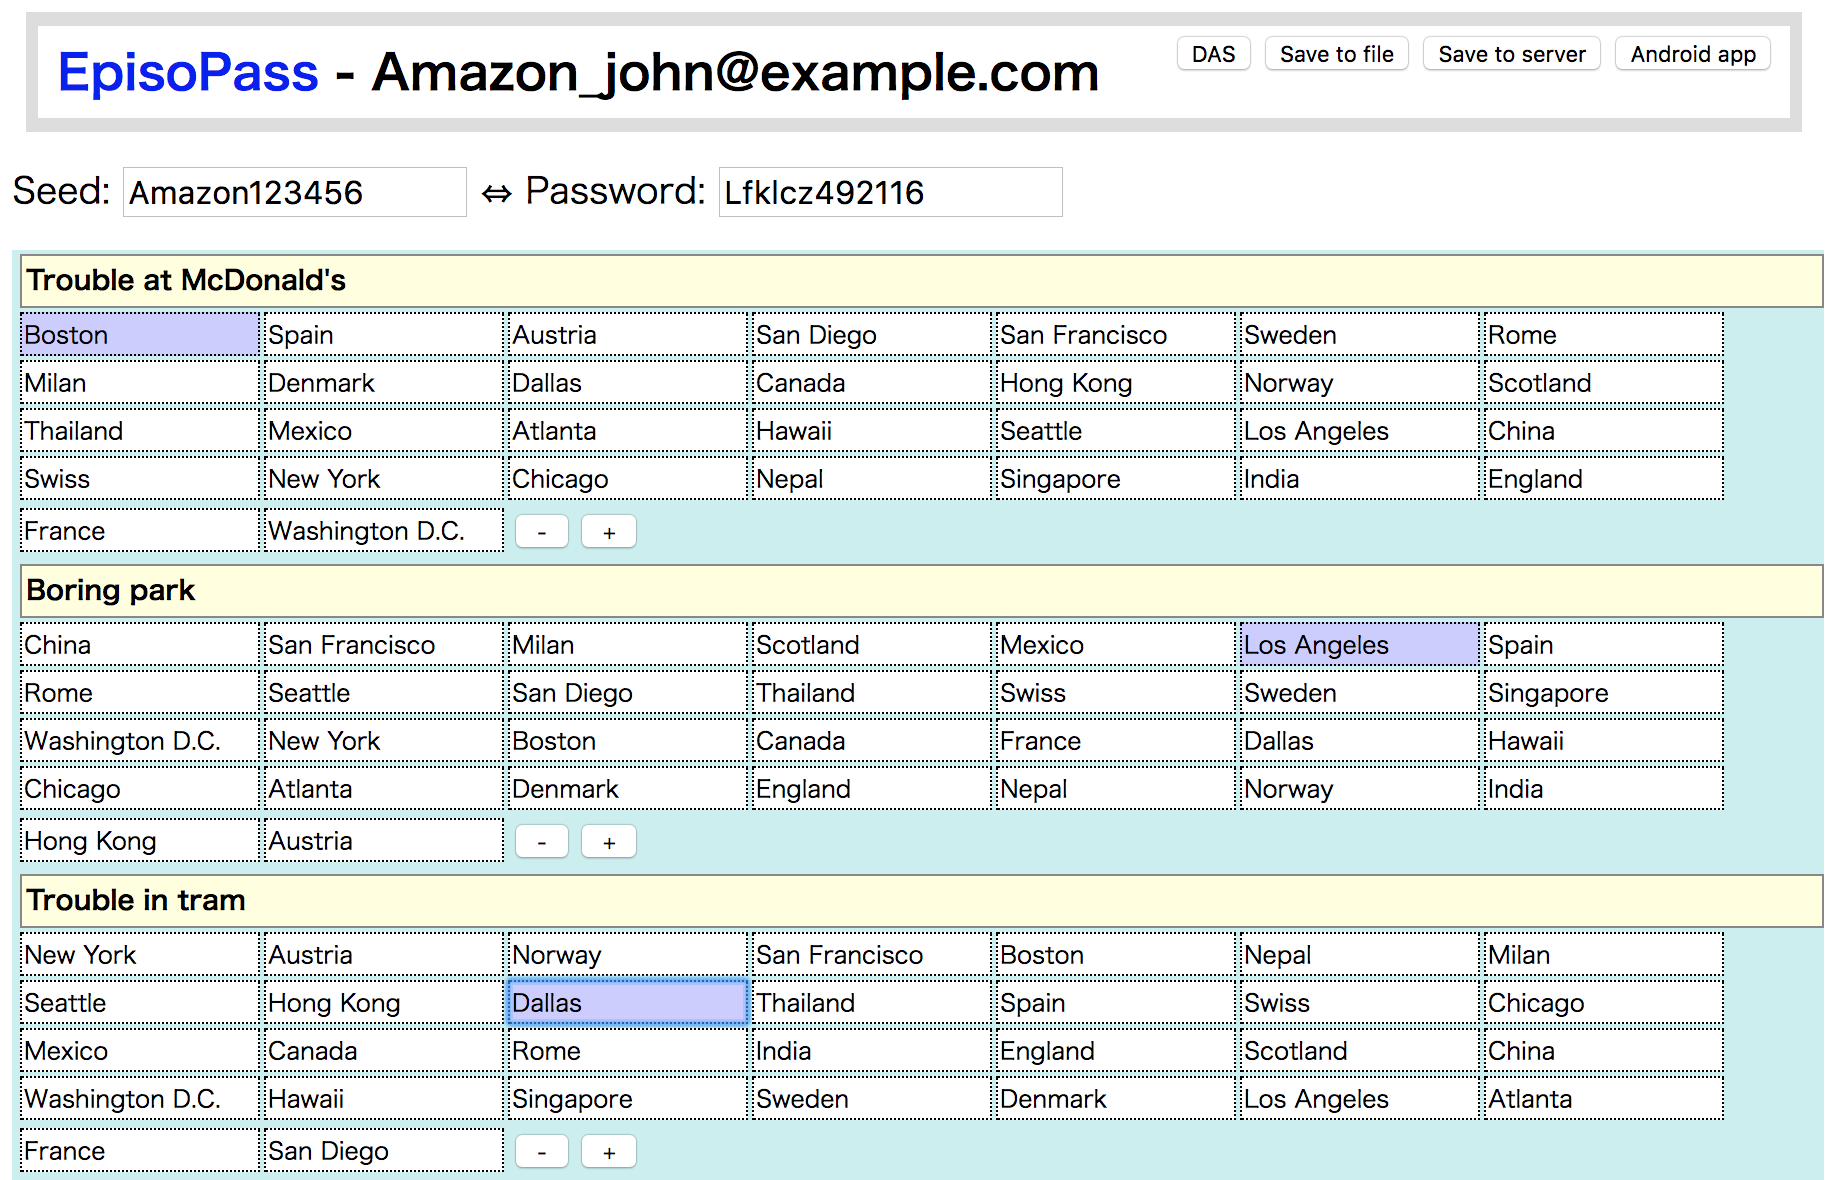
\includegraphics[width=12cm,bb=0 0 1832 1180]{figures/JohnEpisodes.png}
  \caption{EpisoPass window}
  \label{JohnEpisodes}
\end{figure}

After selecting the correct answers
(``Boston'', ``Los Angeles'', etc.) on the EpisoPass page,
the user can click the ``DAS'' button on the top-right portion of the
EpisoPass page,
%
% After cliking the button,
% a page for registering the DAS pattern id shown to ther user, and
and the user can specify his DAS patten on the registration page.

\begin{figure}[H]
  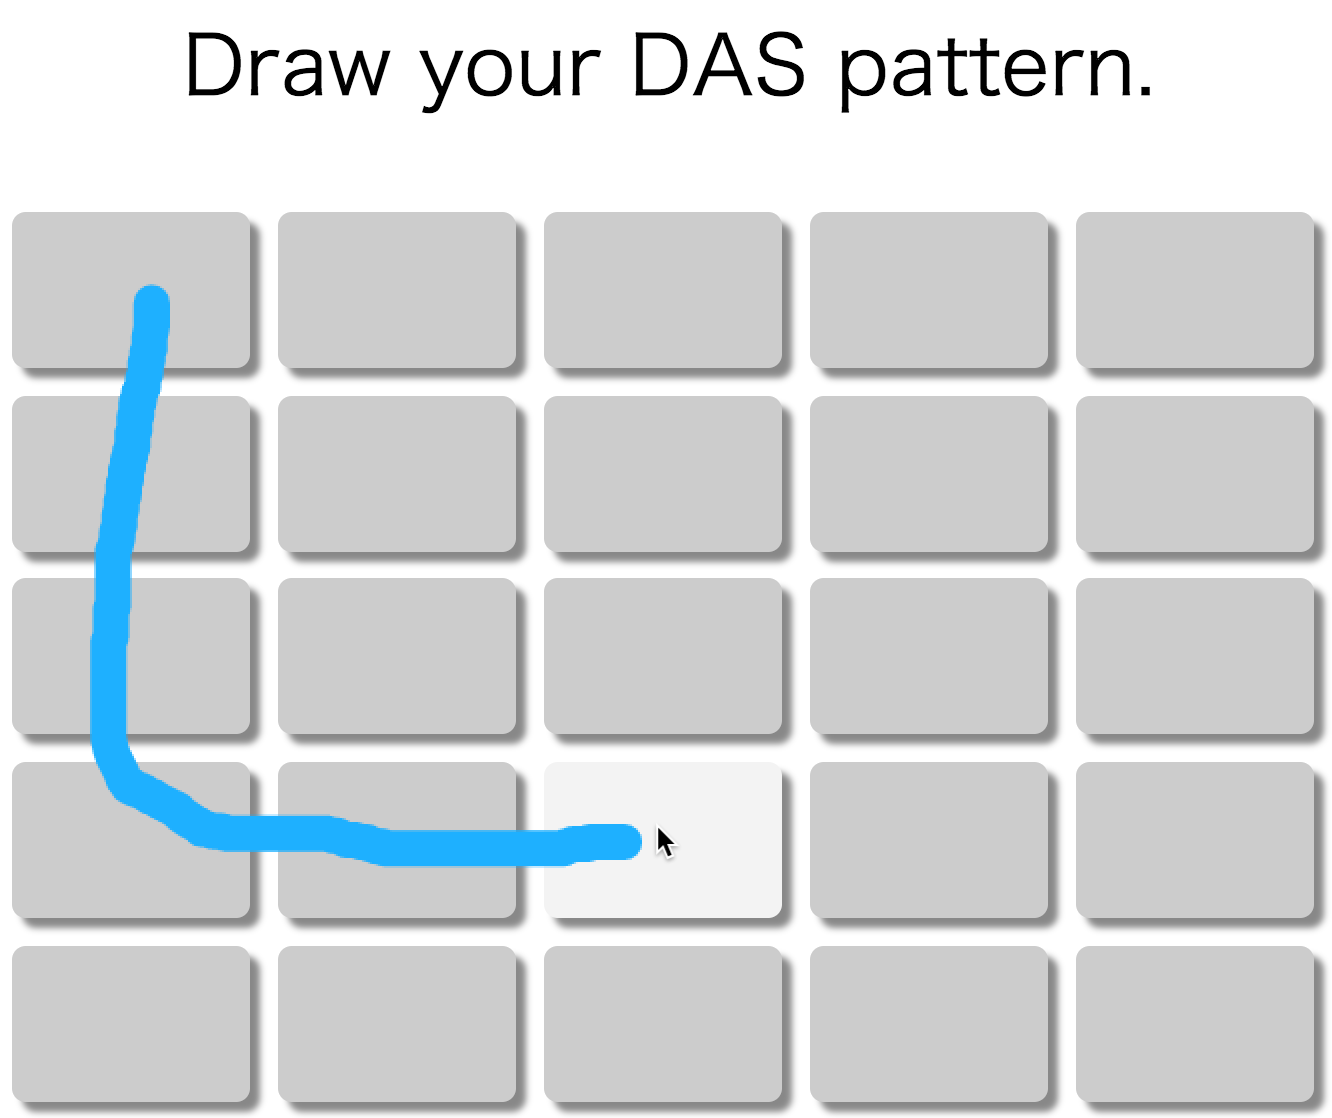
\includegraphics[width=12cm,bb=0 0 1332 1118]{figures/DASRegister.png}
  \caption{Registring the DAS pattern}
  \label{DASRegister}
\end{figure}

If the user wants to use a U-shape as the secret pattern,
he can draw the shape shown in Figure \ref{draw}
on the registration window.
%
After finishing the registration drawing, the candidate answers fo the EpisoPass is
shuffled so that the correct answers represent the specified pattern.

\subsection{Registering questions and answers}

Questions and answer candidates can be edited interactively on the
EpisoPass page (Figure \ref{EpisoPass}).
However, creating many questions and answer candidates is hard because
people usually feel it hard to remember secret episodes.
%
To help people easily create EpisoPass problems,
we have provided a special page for easy problem creation
(Figure \ref{Easy}).

\begin{figure}[H]
  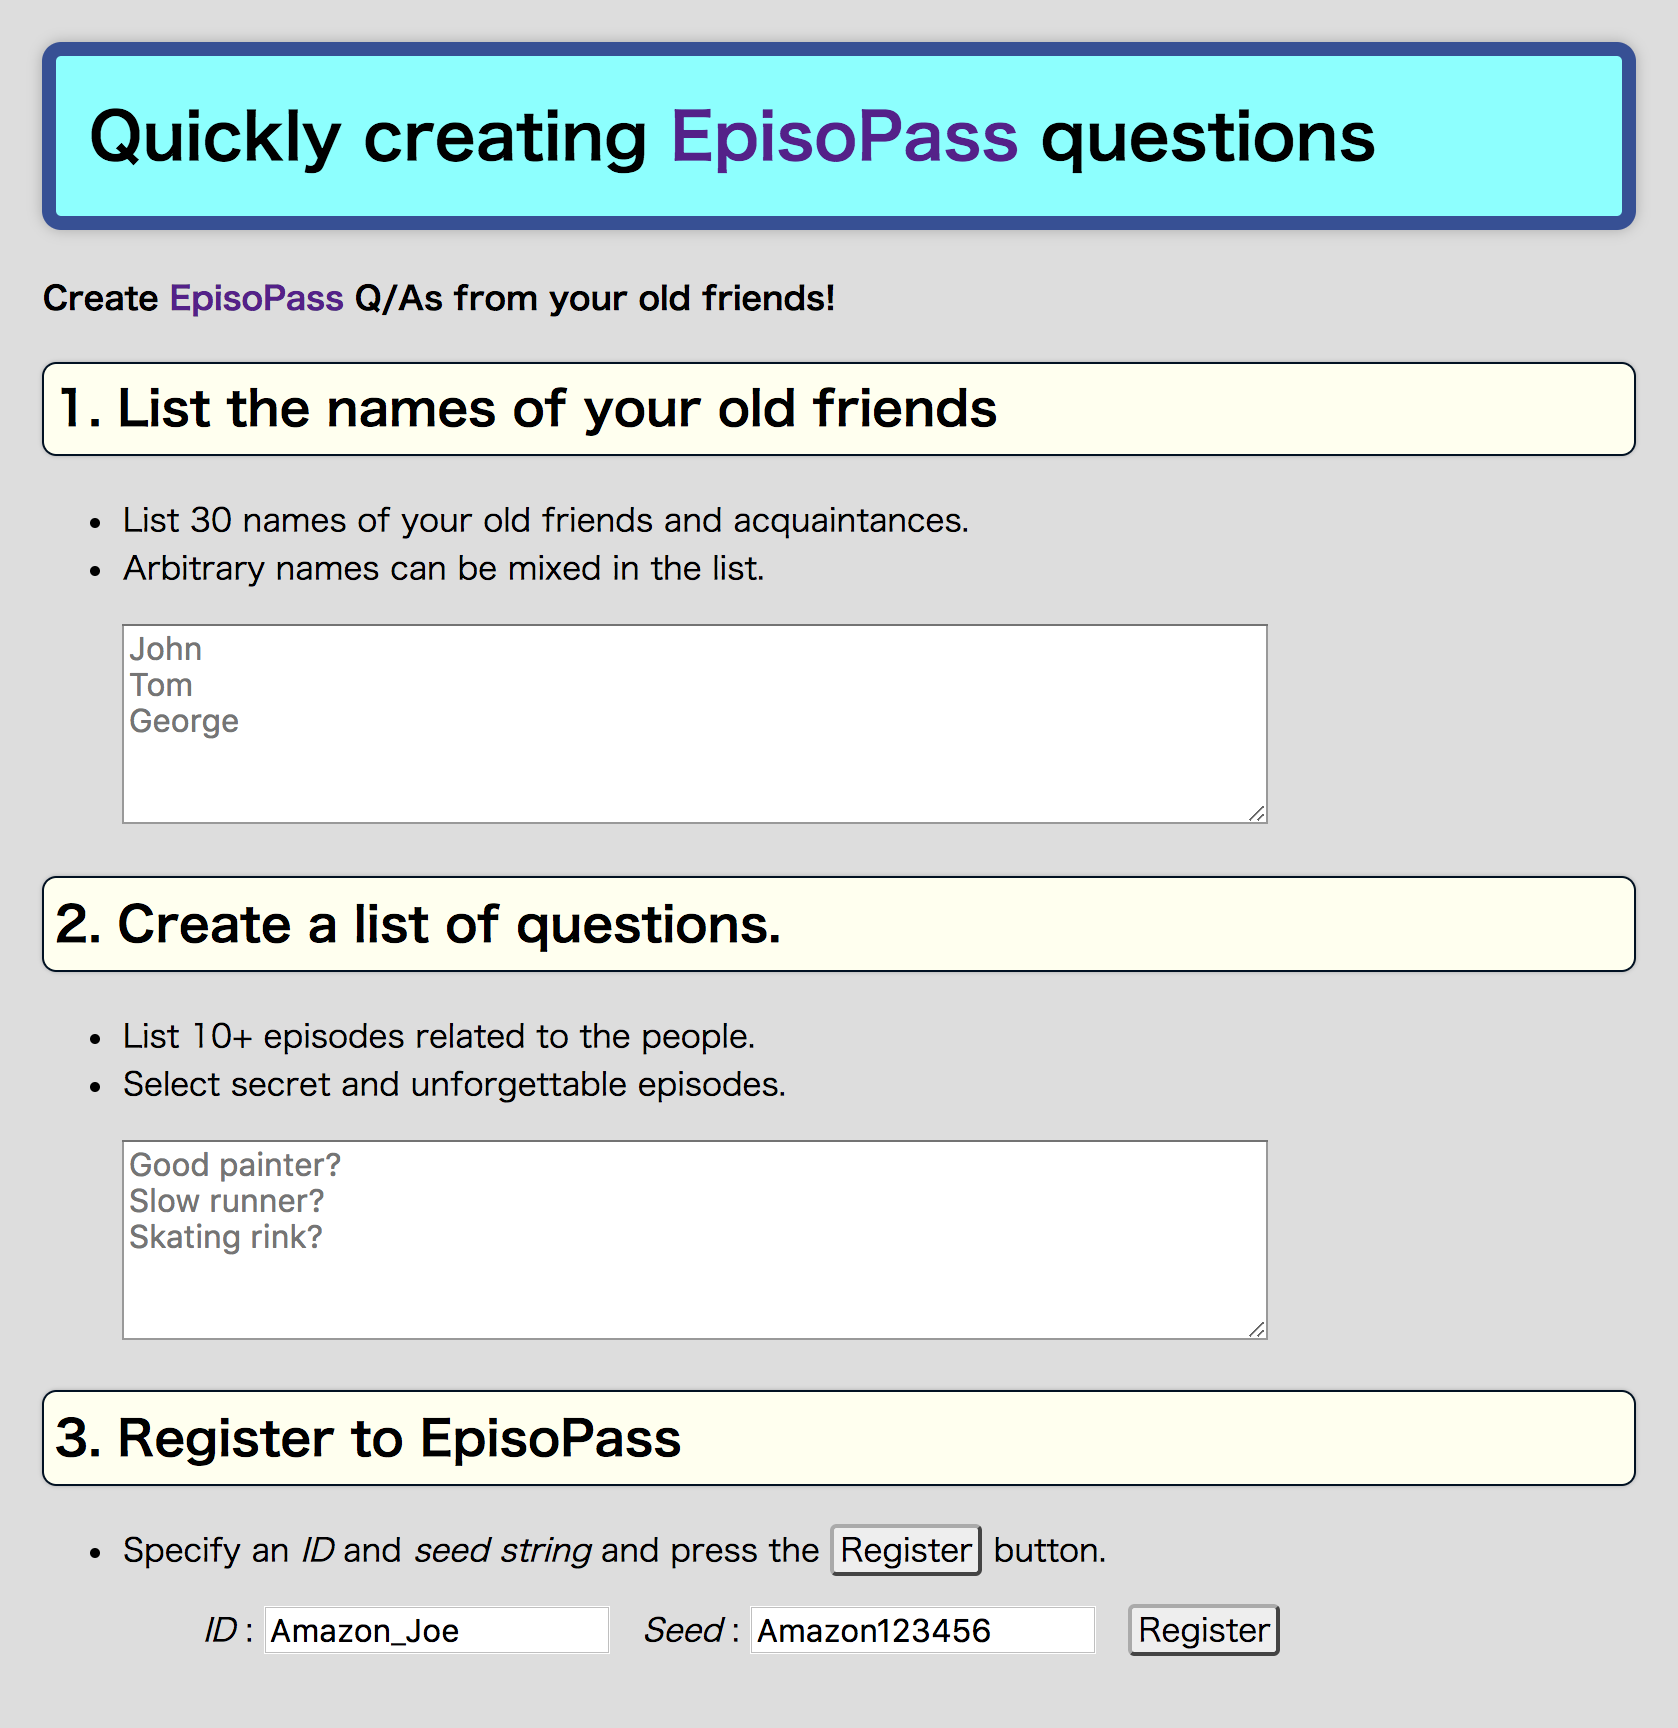
\includegraphics[width=12cm,bb=0 0 1332 1118]{figures/Easy.png}
  \caption{Easily creating problems}
  \label{Easy}
\end{figure}

First, users enter the names of their old friends and acquaintances.
After creating a list of such names,
the users are asked to enter special episodes of the people.
For example, if the user remembers that Tom was
very good at drawing, he can add a question
``Good painter?'' to the list, assuming Tom is the correct answer.

Remembering a special old episode is fairly hard for most people, but
remembering an attribute of an old friends seems to be much easier.

\section{Evaluation}

The authors have been using EpisoPass for more than 5 years, and
using EpisoDAS for about an year.
No formal evaluation has been performed so far, but
important impressions have been observed during the period.

速度

\section{Discussion}

速度
拡張機能を利用すると
記憶しているパスワード入力よりも高速なぐらいで入力できる


覚えることが要らなくなった
公開しても大丈夫
  ググれる
* マスターパスワードが要らない

問題づくり

使い回しが駄目

サイトごとのカスタマイズが大変

覗き見は危険

ひとつのHTML

強度



Using a conventional DAS system, users should be carefull about
remembering the DAS pattern.
DAS patterns may be more easily remembered than password texts,
but there is always some risks about forgetting them.
Using EpisoDAS, users can easily remember the DAS pattern
just by reading the questions and answers.
Users can be very sure that they will never forget the pattern,
because the pattern can be retrieved by answering the questions.


EpisoDAS is the combination of EpisoPass and DAS-based authentication methods.
A user can generate a password using his episodic memories, or
he can generate a password using the DAS pattern he remembers.
%
EpisoDAS has the advantages of both of the systems: i.e.
users never forget how to generate the password, and
users can quickly generate his password.

\section{Conclusion}

% \begin{acks}
% \end{acks}

% \bibliographystyle{ACM-Reference-Format}
\bibliography{sample-bibliography}

\end{document}
